\documentclass[a4paper,11pt]{article}
\usepackage{xunicode}
\usepackage[french]{babel}
\usepackage{graphicx}
\graphicspath{ {./illustrations/} }


\begin{document}


	\begin{titlepage}
		\begin{center}
			\vspace{0.5cm}

			\Huge
			\textbf{PicToShare}

			\vspace{0.5cm}
			\textbf{Documentation utilisateur}

			
\includegraphics[width=\textwidth]{PTS_icon}

			\Large
			Guillaume Chauveau \\
			Anaïs Doidy \\
			Steven Hue \\
			Nathan Moureaux\\

			\vspace{1cm}
			Encadrant : Bertrand Coüasnon

			\vspace{1cm}
			2020-2021

		\end{center}

	\end{titlepage}


	\section{Introduction}

	PicToShare (PTS) est une application développée pour MacOS permettant à l'utilisateur de scanner ou d'importer, puis de classifier rapidement des documents. L'import du document peut se faire depuis une photo prise avec un appareil mobile Apple via la technologie Continuity, ou bien depuis un fichier déjà présent sur l'ordinateur. Une fois le fichier importé, un traitement est effectué en fonction des paramètres choisis, et éventuellement de l'AppleScript associé. Le fichier final est annoté puis classé dans un dossier PTS dédié, le but étant de retrouver facilement ce document, via une recherche Spotlight par exemple.


	\section{Déroulement d'une utilisation}

	Une fois l'application installée, il y a deux manières d'interagir avec PTS : à partir d'une prise de photo via un appareil Apple, ou à partir d'un fichier déjà présent sur l'ordinateur.

	\subsection{Prise de photo d'un document}

	Afin de prendre une photo d'un document, un clic sur l'icône de l'appareil photo vous affichera les appareils disponibles. Une fois l'appareil sélectionné, le mode photo sera automatiquement activé sur celui-ci, et il ne vous restera plus qu'à prendre la photo. Elle sera automatiquement transférée vers l'ordinateur.
		\begin{figure}[h!]
			\centering
			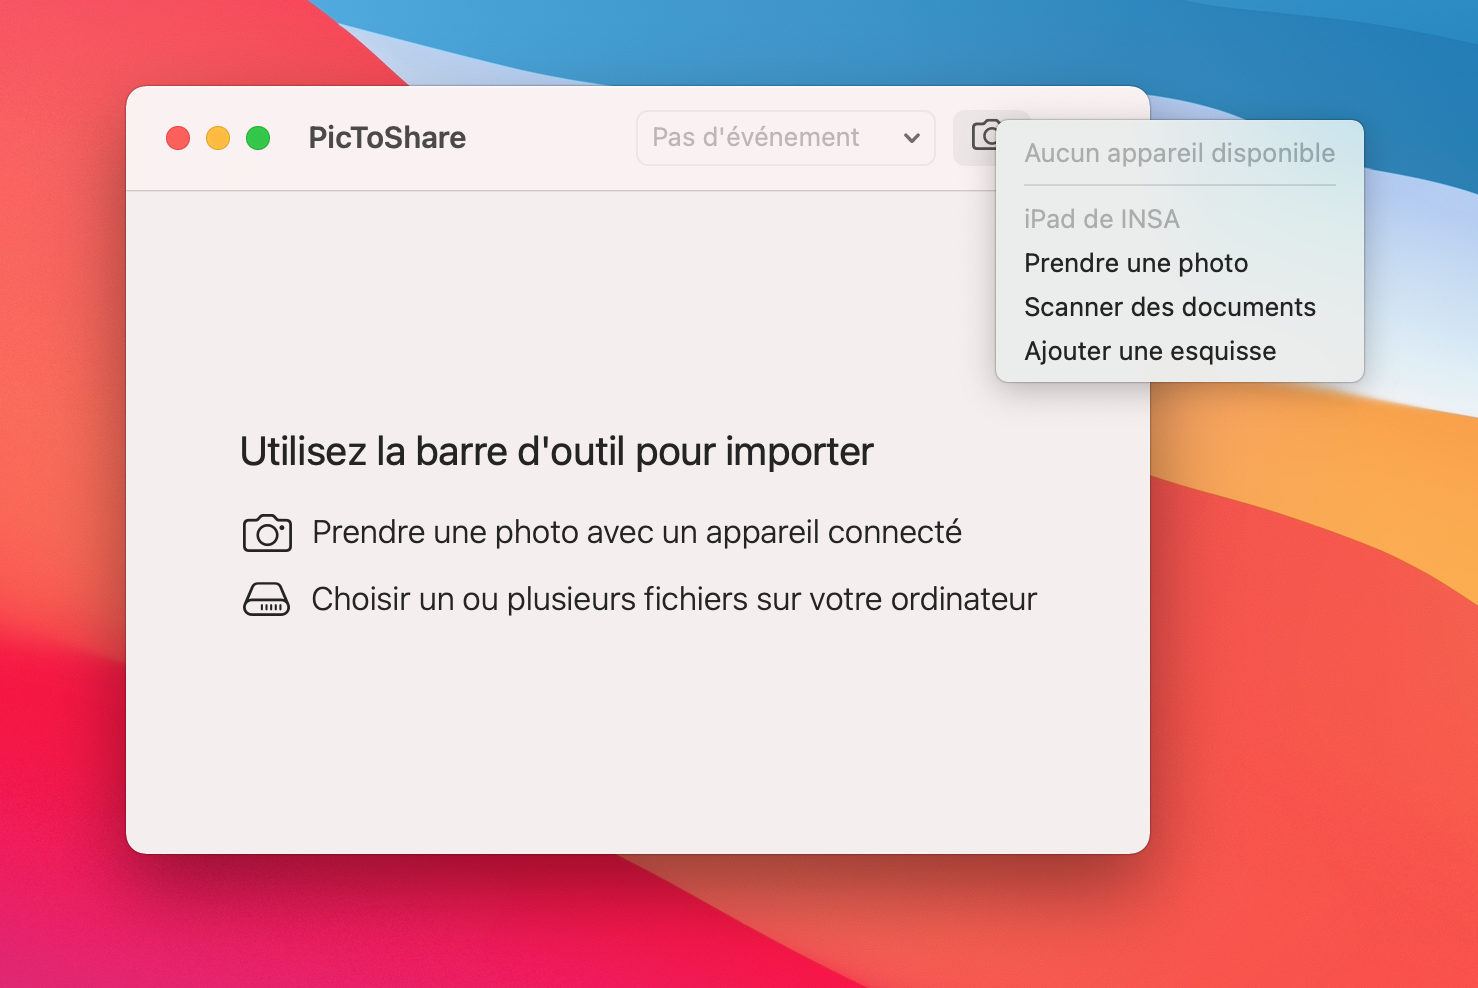
\includegraphics[width=11cm]{Continuity}
			\caption{Prise de photo via Continuity}
		\end{figure}


	\subsection{Import d'un fichier présent sur l'ordinateur}

	Si le document se trouve déjà sur votre ordinateur, un clic sur l'icône du disque dur vous affichera une fenêtre de sélection de fichier. Vous pouvez sélectionner plusieurs fichiers en même temps.
		\begin{figure}[h]
			\centering
			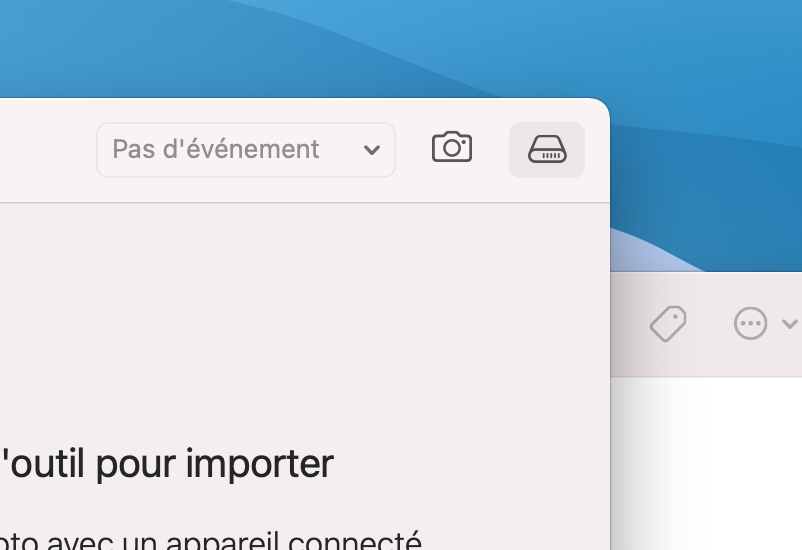
\includegraphics[width=8cm]{DD_import}
			\caption{Selection d'un fichier présent sur le Mac}
		\end{figure}

	Il est aussi possible de sélectionner directement le ou les fichiers à importer depuis Finder, avec un clic droit puis "PicToShare: importer", afin d'initialiser le processus d'importation.

	\begin{figure}[h]
		\centering
		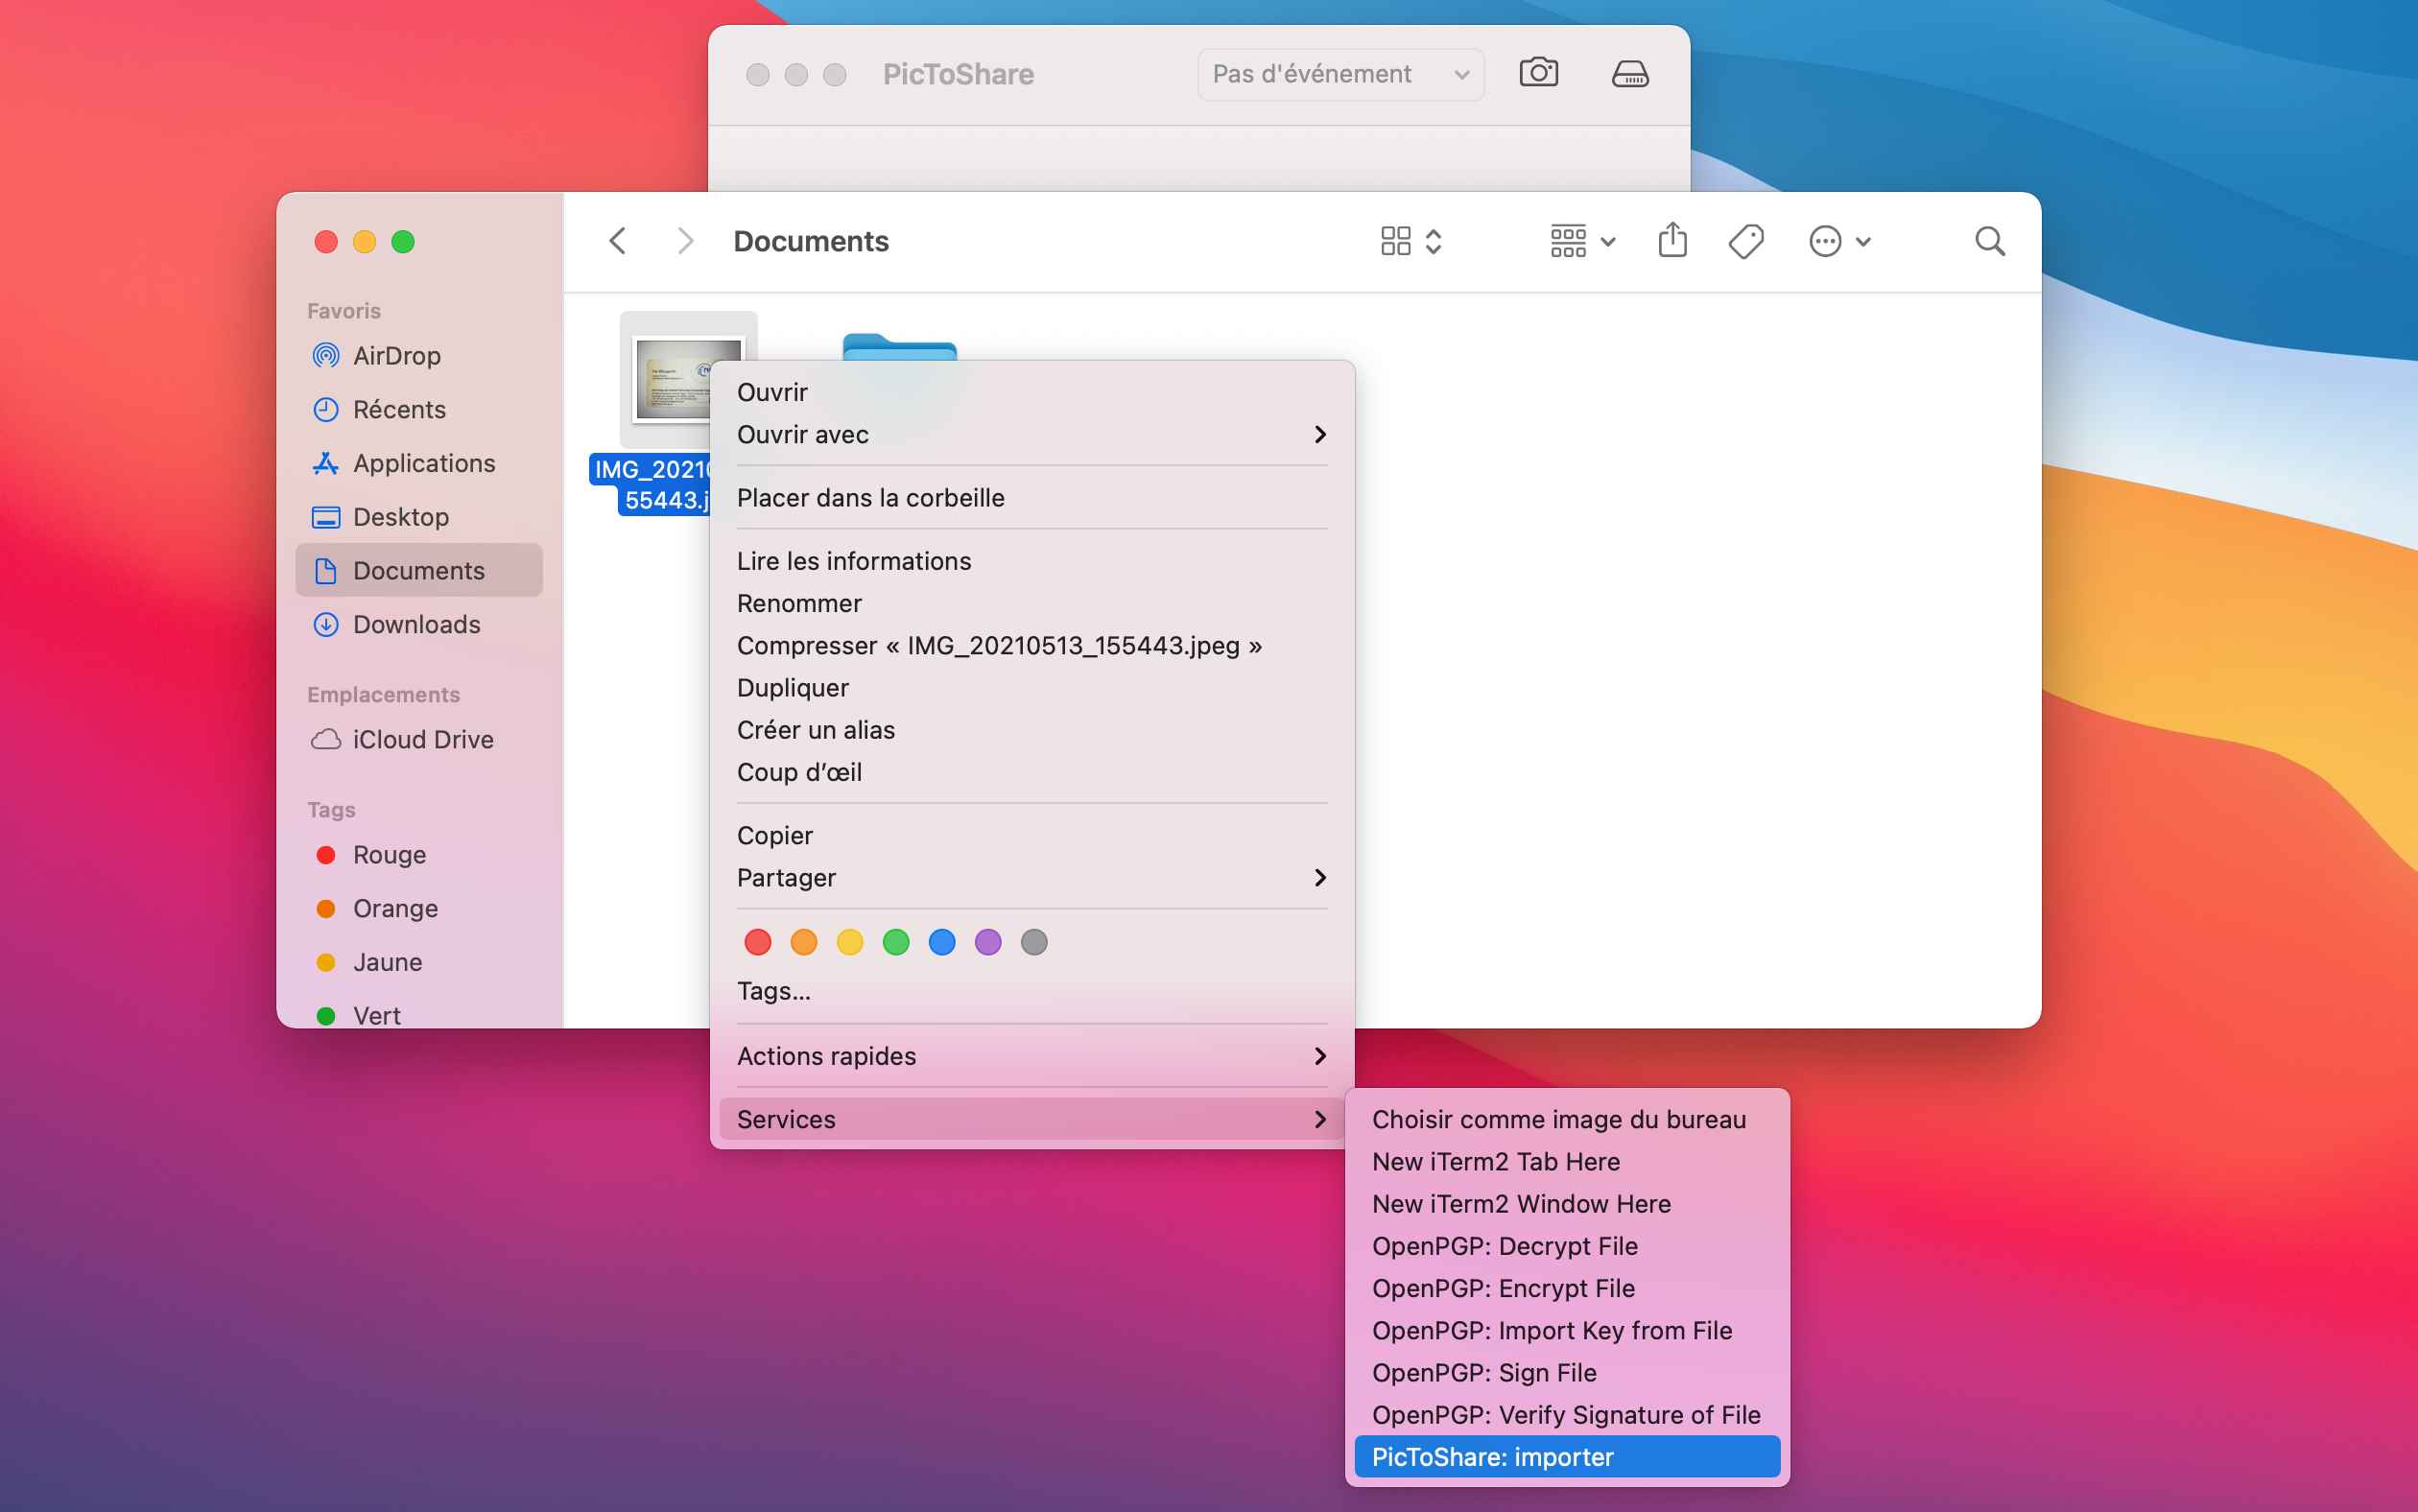
\includegraphics[width=13cm]{Right_click_shortcut}
		\caption{Importation directement depuis le Finder}
	\end{figure}

	\subsection{Choix du type de fichier et d'événement}

	Une fois le document importé, vous disposez d'une prévisualisation de celui-ci sur la gauche (1). Il vous faudra maintenant sélectionner les paramètres représentant votre document.

	\begin{itemize}

		\item Type de document (obligatoire) : sur la droite se trouve une liste de type de document (2), correspondant à la "nature" de celui-ci.
		\item Type d'événement (facultatif) : en haut se trouve une liste déroulante d'événements (3), dont le but est d'associer au document à traîter le contexte dans lequel vous vous trouvez à l'instant (une réunion chez une certaine entreprise par exemple). Pour une meilleure expérience utilisateur, le dernier événement utilisé est automatiquement sélectionné pour la prochaine importation, et il est possible d'ajouter un événement à la volée directement depuis la fenêtre d'importation (4). Si vous ne voulez pas associer d'événement, sélectionnez "Pas d'événement".

	\end{itemize}

	\begin{figure}[h]
		\centering
		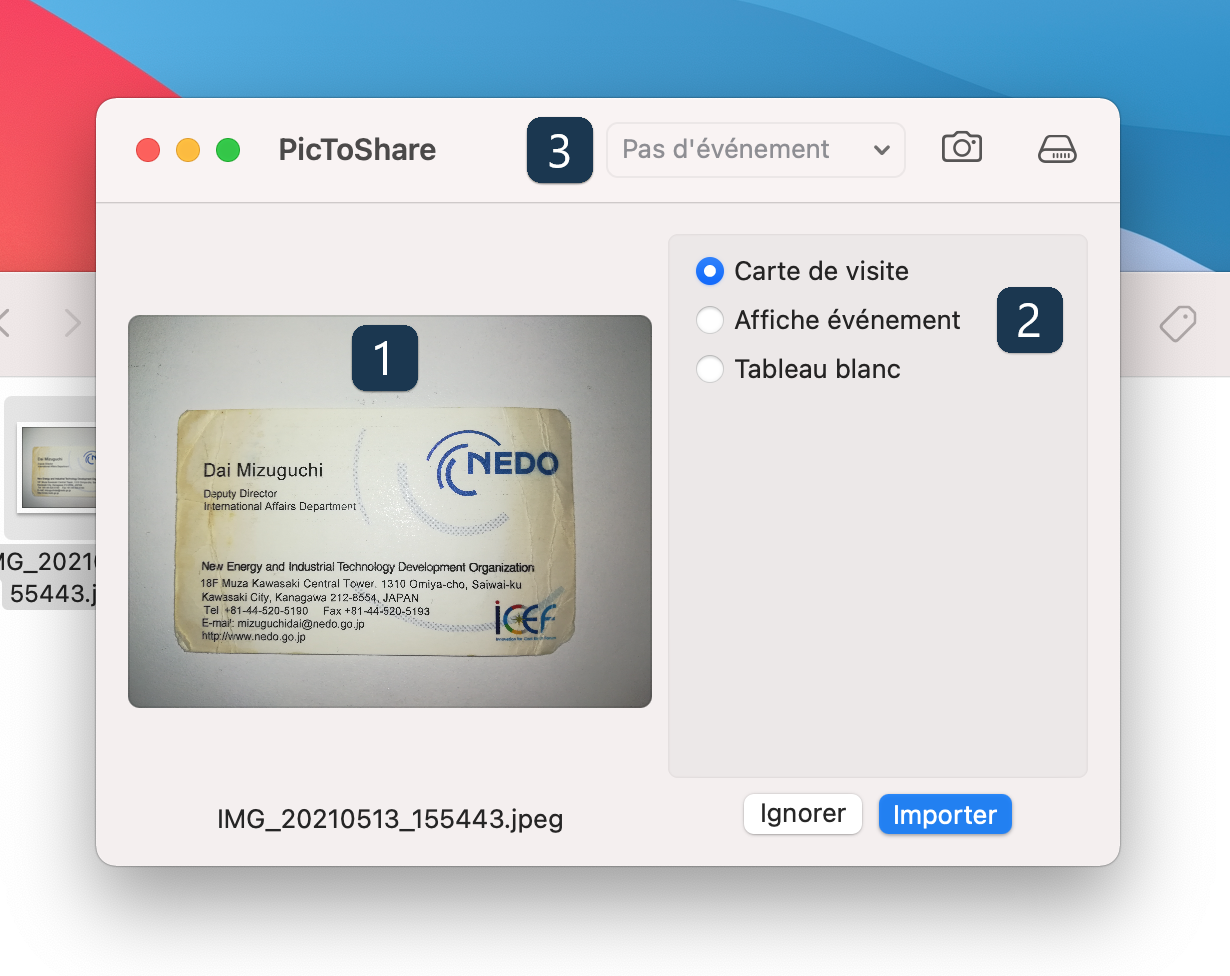
\includegraphics[width=12cm]{Importation_standby}
		\caption{Interface d'importation}
	\end{figure}

	\begin{figure}[h]
		\centering
		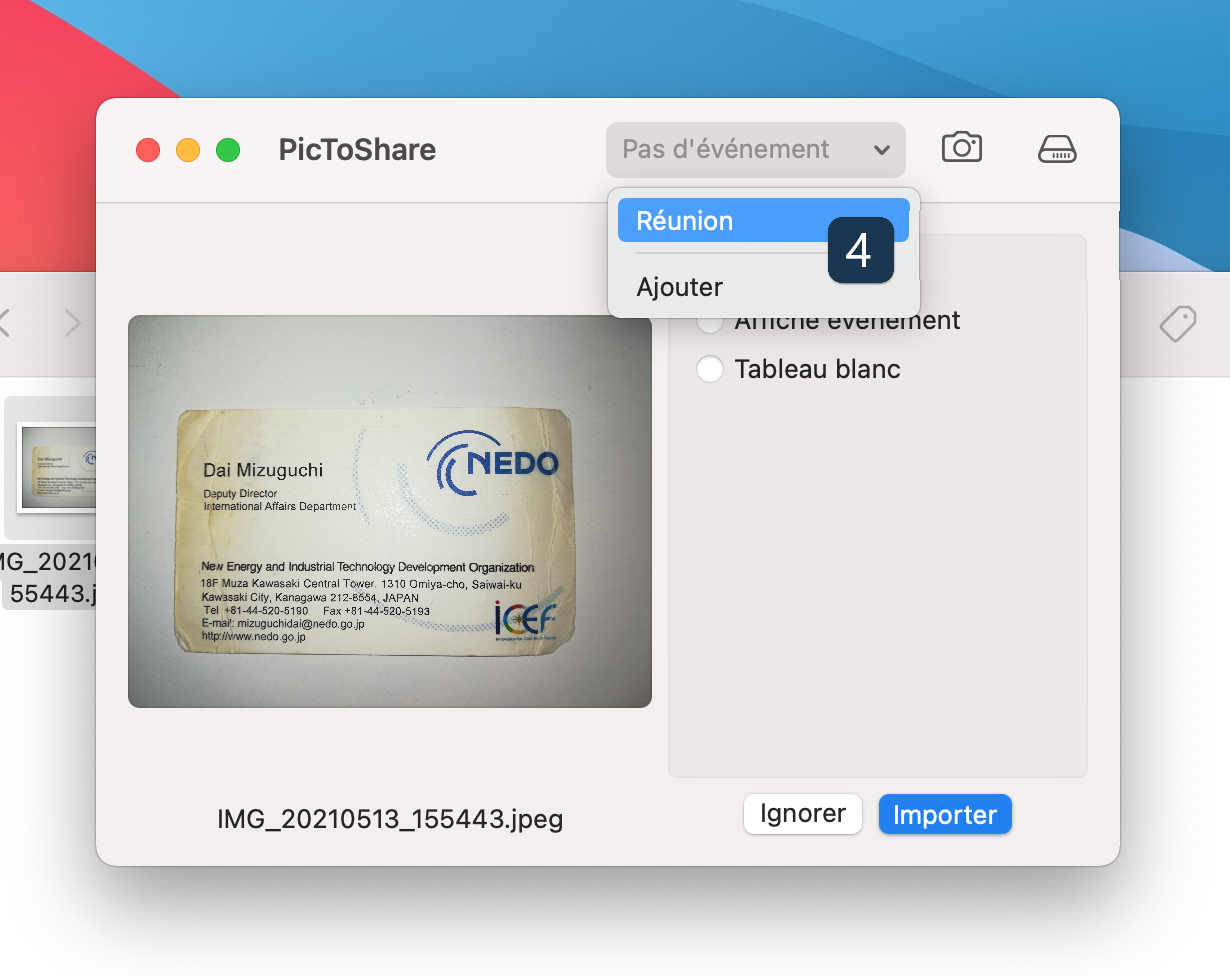
\includegraphics[width=11cm]{Importation_event}
		\caption{Choix de l'événement}
	\end{figure}


	Sur l'exemple, le document à traîter est une carte de visite, prise pendant une réunion avec l'entreprise NEDO.

	\subsection{Retrouver ses fichiers}
	Un dossier intitulé "PTSFolder" est créé dans Documents, dans lequel se trouve un dossier pour chaque type de document, contenant les fichiers ou leur raccourci. Il est aussi possible de les retrouver via une recherche Spotlight sur le type de document, type d'événement ou autres annotations qui seront détaillées un peu plus bas.



	\section{Paramétrage}
	Les types de documents et événements sont la clé d'une utilisation efficace de PTS, et sont paramétrables dans Preferences....
	\begin{figure}[h!]
		\centering
		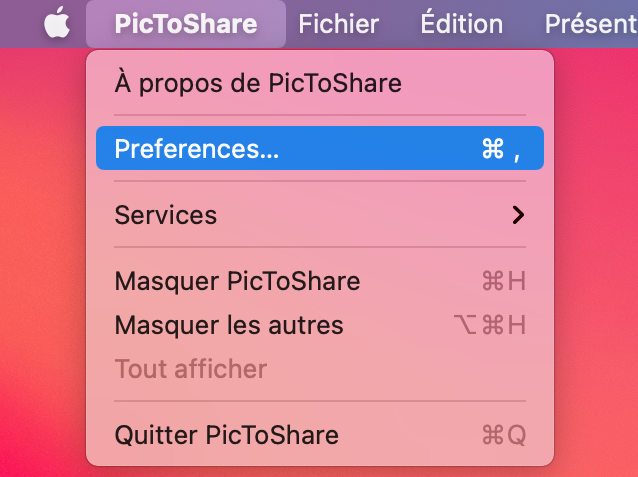
\includegraphics[width=5cm]{Preferences}
		\caption{Preferences}
	\end{figure}


	\subsection{Paramètrage des types de documents}
	C'est ici que vous pouvez ajouter, retirer(1), et modifier(2) les types de documents que vous allez manipuler.
	Voici les différents paramètres avec lesquels vous pouvez interagir :

	\begin{itemize}
		\item Nom : le nom que vous donnez à votre type de document. C'est également le nom du sous-dossier dans PTSFolder où seront rangés tous les documents du même type. Si vous le modifiez, le nom du dossier sera automatiquement modifié lui-aussi.

		\item Script de traitement : il est possible de faire appel à une application externe à PTS afin de traîter plus en profondeur votre document. Par exemple, vous voudriez peut-être utiliser un OCR afin que le texte soit selectionnable et interprétable par votre ordinateur, s'il s'agit d'un document contenant de l'écriture. Pour se faire, il faut que vous fournissiez à PTS un AppleScript rédigé par vos soins. Un script pour l'application Tesseract et un autre pour Pages sont fournis avec l'application, et libre à vous d'utiliser vos logiciels de traîtement favoris en fonction de vos besoins.\\
		En fonction de l'application externe que vous allez utiliser, PTS récupèrera soit le fichier original modifié, soit un nouveau fichier issu de l'original. Il vous est possible de garder une copie de l'original (première option), et/ou de se débarasser de l'original si le script produit d'autres fichiers (deuxième option). Aussi, si un nouveau fichier est créé, PTS ne pourra le détecter seulement s'il possède le même nom que l'original, à l'extension près. Assurez-vous que le résultat produit soit conforme à cette contrainte.

		\item Annotation de contexte : ce paramètre contrôle l'ajoût d'annotations dans le fichier final. Dans la version actuelle de PTS, seulement deux types d'annotations de contexte sont disponibles :
			\begin{itemize}
				\item[-] Événement en cours : ajoute le ou les événements du calendrier se déroulant actuellement. Il est possible de choisir en détail quel calendrier utiliser plus bas.
				\item[-] Géolocalisation : ajoute votre position (pays - ville - nom de lieu)
			\end{itemize}

		\item Intégrations : l'intégration du calendrier permet d'ajouter un lien vers le document dans les notes du ou des événements en cours, en fonction des calendriers sélectionnés.

		\item Calendriers : ce paramètre permet de sélectionner quels calendriers doivent ou ne doivent pas être concernés par l'annotation de contexte "Événement en cours" et l'intégration dans Calendrier.
	\end{itemize}

	\newpage

	\begin{figure}[h!]
		\centering
		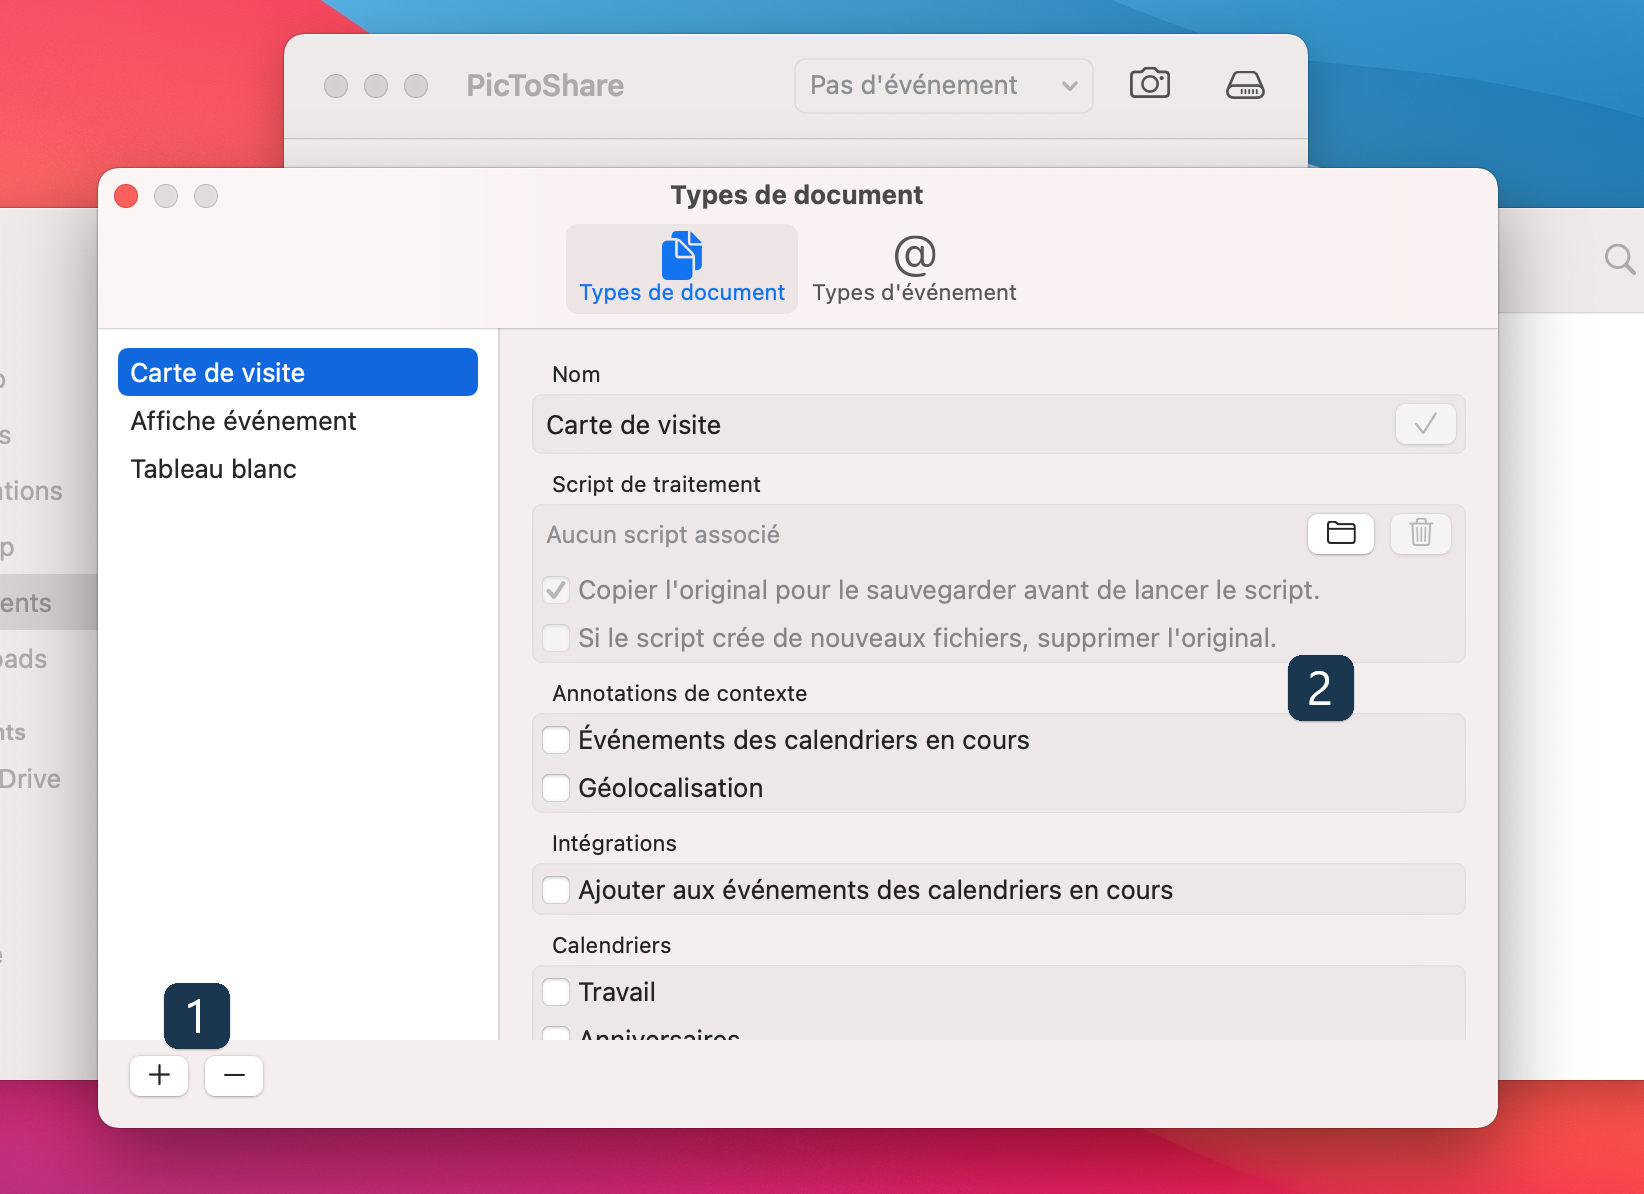
\includegraphics[width=10cm]{Type_de_doc}
		\caption{Fenêtre de paramétrage des types de documents}
	\end{figure}

	\subsection{Paramétrage des types d'événements}
	C'est ici que vous pouvez ajouter, retirer et modifier les types d'événement que vous allez manipuler.
	Voici les différents paramètres avec lesquels vous pouvez interagir :
	\begin{itemize}
		\item Nom : le nom que vous donnez à votre type d'événement
		\item Annotations de contexte : identique aux types de documents
		\item Intégrations : \textit{idem}
		\item Calendriers : \textit{idem}
	\end{itemize}

	\begin{figure}[h!]
		\centering
		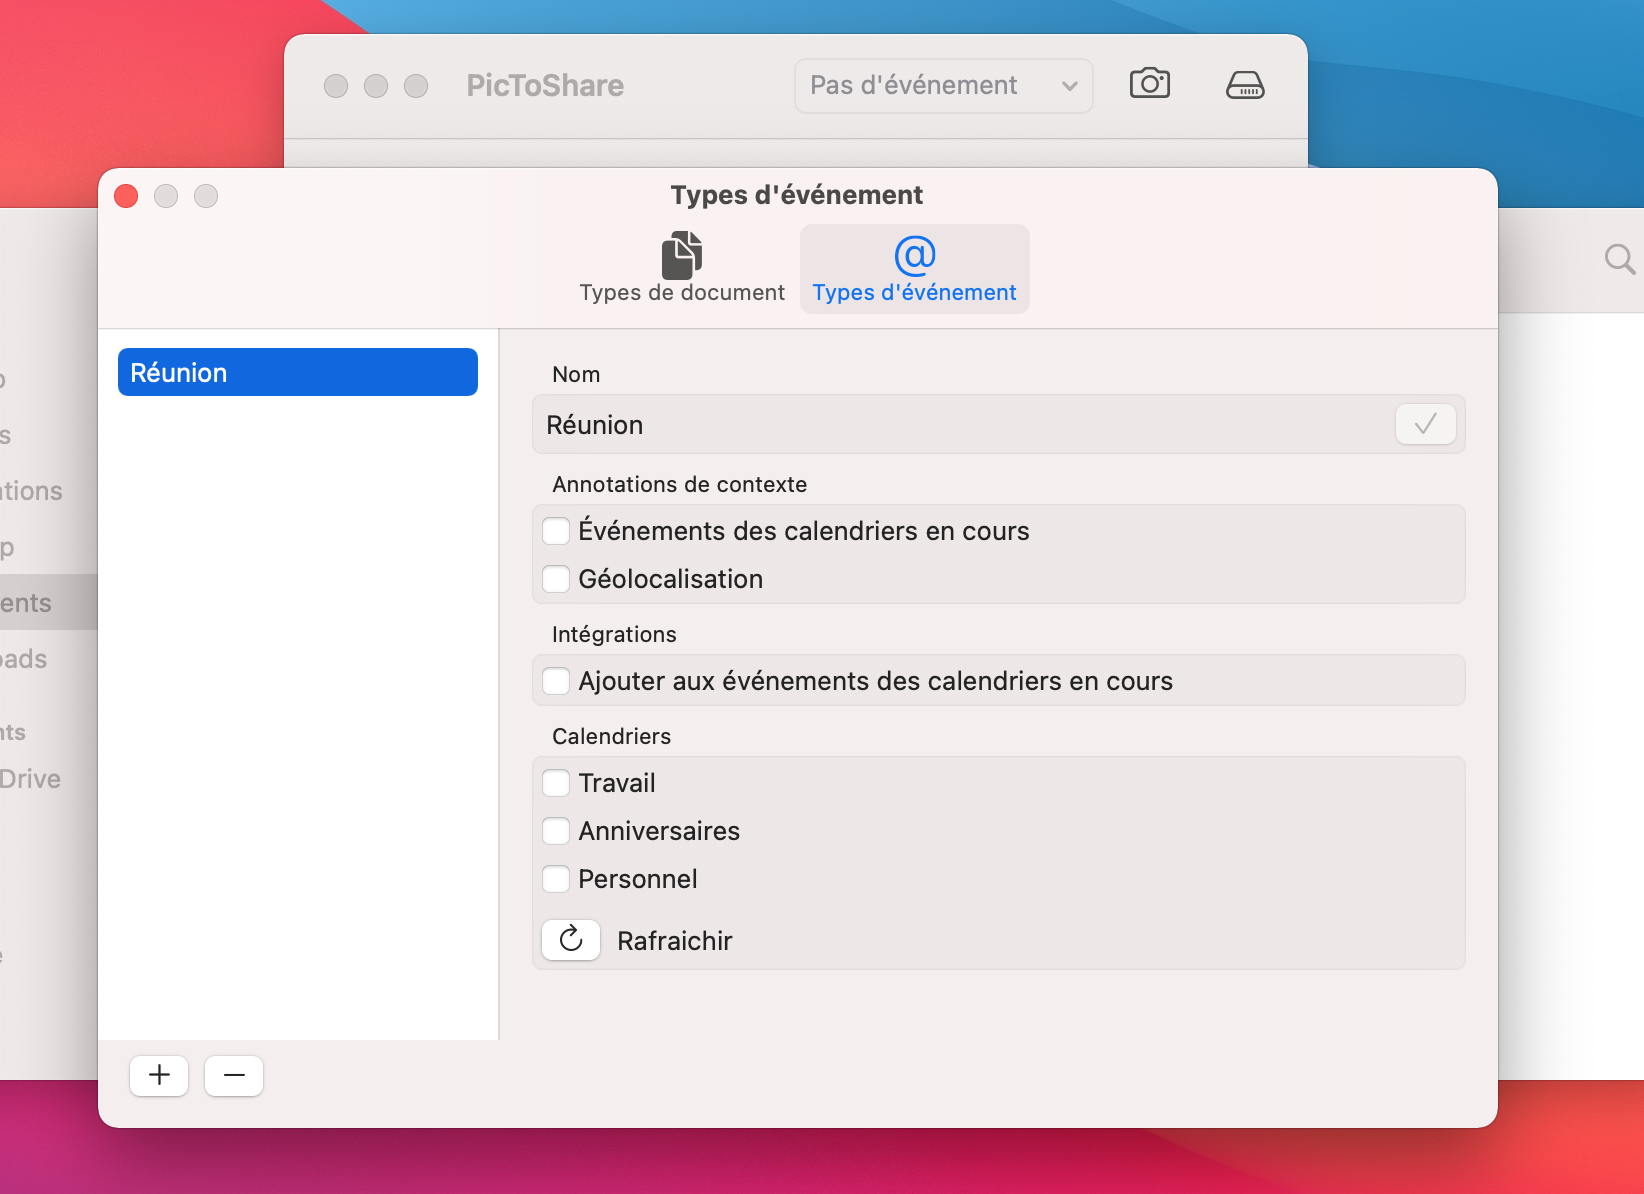
\includegraphics[width=8cm]{Type_d_event}
		\caption{Fenêtre de paramétrage des types d'événements}
	\end{figure}

	\subsection{Union des paramètres}
	Certains paramètres peuvent être présents à la fois pour le type de document et le type d'événement. Lors du traitement, une union de ces paramètres est effectuée pour ne pas produire de doublons. Par exemple, si l'intégration dans Calendrier est sélectionnée pour le type de document et le type d'événement, il n'y aura qu'un seul lien vers le fichier dans Calendrier. Autre exemple, si dans l'un l'annotation de Calendrier est sélectionnée, et que dans l'autre la géolocalisation l'est, le fichier produit possédera les deux annotations.


	\section{Annotation des fichiers}
	Lorsque PTS traîte un fichier, il l'annote en plaçant des mots dans la propriété mots-clés du fichier, qui sont utilisés par Spotlight afin l'indexer. Voici une liste du contenu que vous pouvez retrouver dans les mots-clés d'un fichier :
	\begin{itemize}
		\item Type de document
		\item Type d'événement
		\item Géolocalisation
		\item Événement en cours dans le calendrier
	\end{itemize}

	\begin{figure}[h!]
		\centering
		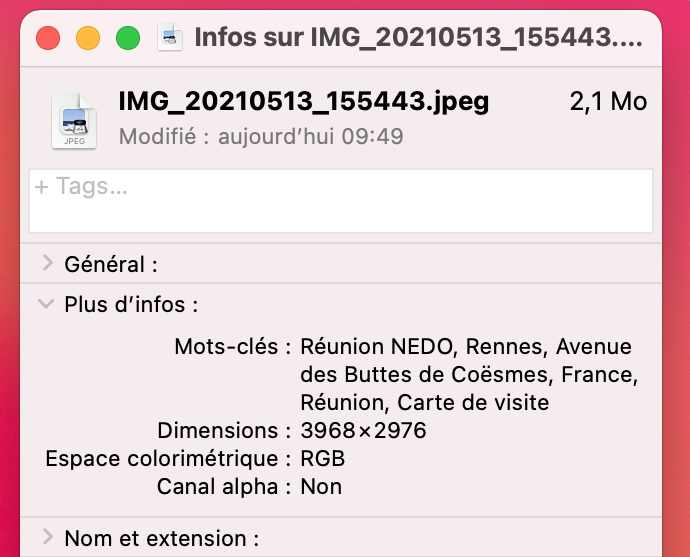
\includegraphics[width=10cm]{Mots-cles}
		\caption{Mots-clés d'un document traîté}
	\end{figure}

	Ces mots-clés ne sont pas supprimables ou modifiables depuis Finder, mais d'autres applications ou le Terminal le permettent.

\end{document}dis
